\documentclass[14pt]{extbook}
\usepackage{multicol, enumerate, enumitem, hyperref, color, soul, setspace, parskip, fancyhdr} %General Packages
\usepackage{amssymb, amsthm, amsmath, bbm, latexsym, units, mathtools} %Math Packages
\everymath{\displaystyle} %All math in Display Style
% Packages with additional options
\usepackage[headsep=0.5cm,headheight=12pt, left=1 in,right= 1 in,top= 1 in,bottom= 1 in]{geometry}
\usepackage[usenames,dvipsnames]{xcolor}
\usepackage{dashrule}  % Package to use the command below to create lines between items
\newcommand{\litem}[1]{\item#1\hspace*{-1cm}\rule{\textwidth}{0.4pt}}
\pagestyle{fancy}
\lhead{Progress Quiz 4}
\chead{}
\rhead{Version B}
\lfoot{9187-5854}
\cfoot{}
\rfoot{Spring 2021}
\begin{document}

\begin{enumerate}
\litem{
Solve the radical equation below. Then, choose the interval(s) that the solution(s) belongs to.\[ \sqrt{27 x^2 - 72} - \sqrt{57 x} = 0 \]\begin{enumerate}[label=\Alph*.]
\item \( x \in [2.8,3.3] \)
\item \( x_1 \in [-2.1, -0.5] \text{ and } x_2 \in [3,4] \)
\item \( x \in [-2.1,-0.5] \)
\item \( \text{All solutions lead to invalid or complex values in the equation.} \)
\item \( x_1 \in [0.2, 1.7] \text{ and } x_2 \in [3,4] \)

\end{enumerate} }
\litem{
Solve the radical equation below. Then, choose the interval(s) that the solution(s) belongs to.\[ \sqrt{18 x^2 - 18} - \sqrt{0 x} = 0 \]\begin{enumerate}[label=\Alph*.]
\item \( x_1 \in [-0.2, 1.7] \text{ and } x_2 \in [0,5] \)
\item \( x \in [-0.2,1.7] \)
\item \( \text{All solutions lead to invalid or complex values in the equation.} \)
\item \( x \in [-1.4,0.8] \)
\item \( x_1 \in [-1.4, 0.8] \text{ and } x_2 \in [0,5] \)

\end{enumerate} }
\litem{
Choose the graph of the equation below.\[ f(x) = \sqrt{x + 8} - 7 \]\begin{enumerate}[label=\Alph*.]
\begin{multicols}{2}\item 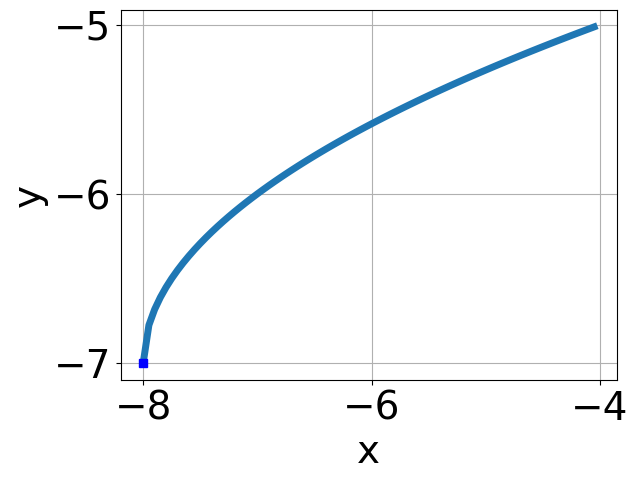
\includegraphics[width = 0.3\textwidth]{../Figures/radicalEquationToGraphAB.png}\item 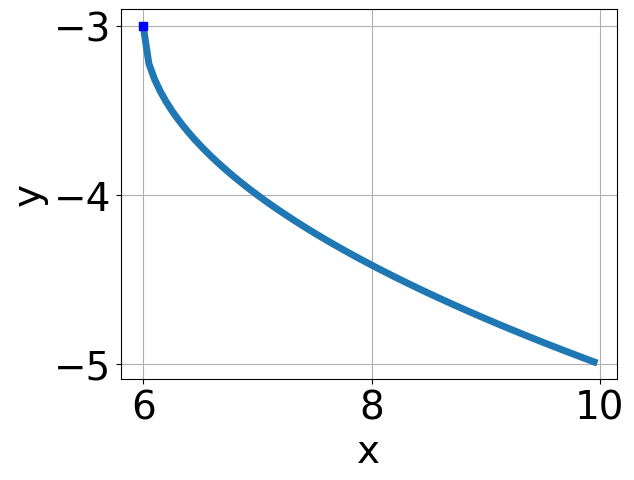
\includegraphics[width = 0.3\textwidth]{../Figures/radicalEquationToGraphBB.png}\item 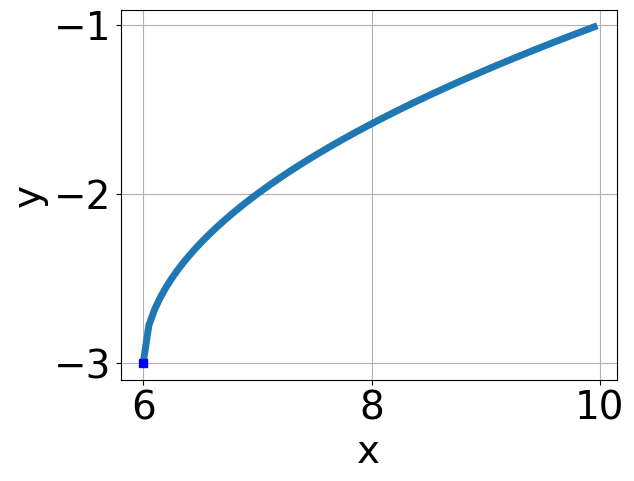
\includegraphics[width = 0.3\textwidth]{../Figures/radicalEquationToGraphCB.png}\item 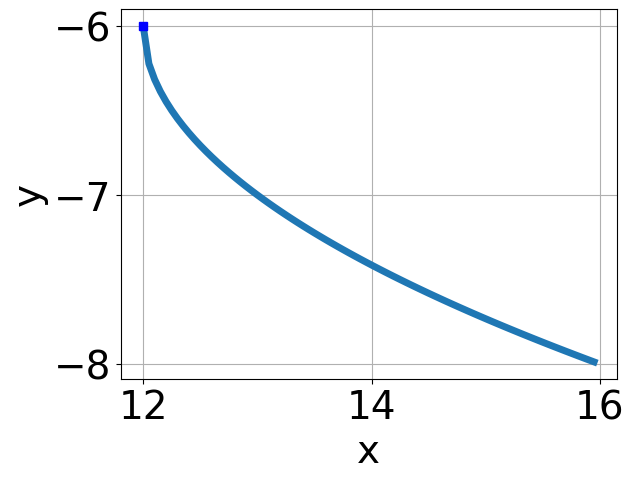
\includegraphics[width = 0.3\textwidth]{../Figures/radicalEquationToGraphDB.png}\end{multicols}\item None of the above.
\end{enumerate} }
\litem{
What is the domain of the function below?\[ f(x) = \sqrt[6]{7 x + 8} \]\begin{enumerate}[label=\Alph*.]
\item \( [a, \infty), \text{ where } a \in [-1.45, -1.05] \)
\item \( (-\infty, a], \text{where } a \in [-1.43, -0.96] \)
\item \( (-\infty, \infty) \)
\item \( [a, \infty), \text{where } a \in [-1.06, -0.66] \)
\item \( (-\infty, a], \text{where } a \in [-1.01, -0.69] \)

\end{enumerate} }
\litem{
Choose the equation of the function graphed below.
\begin{center}
    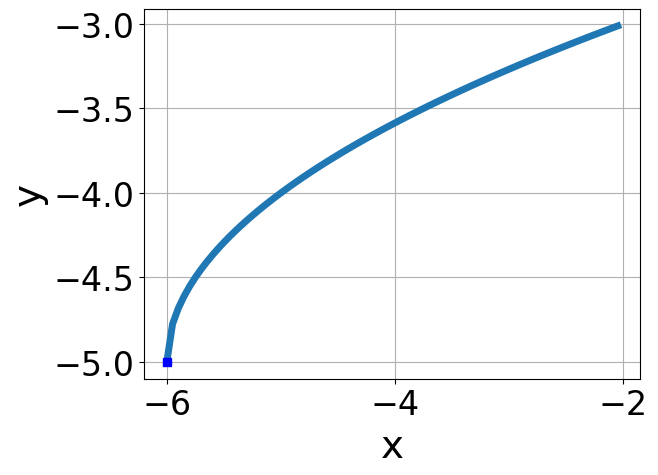
\includegraphics[width=0.5\textwidth]{../Figures/radicalGraphToEquationCopyB.png}
\end{center}
\begin{enumerate}[label=\Alph*.]
\item \( f(x) = \sqrt{x - 14} - 6 \)
\item \( f(x) = - \sqrt{x - 14} - 6 \)
\item \( f(x) = \sqrt{x + 14} - 6 \)
\item \( f(x) = - \sqrt{x + 14} - 6 \)
\item \( \text{None of the above} \)

\end{enumerate} }
\litem{
What is the domain of the function below?\[ f(x) = \sqrt[3]{-4 x + 8} \]\begin{enumerate}[label=\Alph*.]
\item \( \text{The domain is } [a, \infty), \text{   where } a \in [1.3, 3.4] \)
\item \( \text{The domain is } (-\infty, a], \text{   where } a \in [-1.58, 1.15] \)
\item \( (-\infty, \infty) \)
\item \( \text{The domain is } (-\infty, a], \text{   where } a \in [1.77, 2.6] \)
\item \( \text{The domain is } [a, \infty), \text{   where } a \in [-1.3, 0.7] \)

\end{enumerate} }
\litem{
Choose the equation of the function graphed below.
\begin{center}
    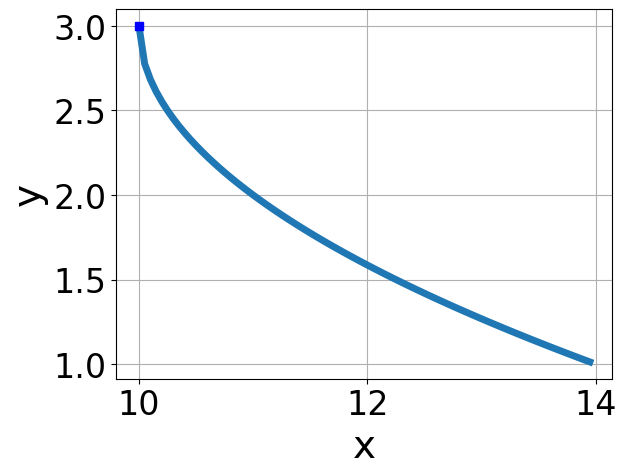
\includegraphics[width=0.5\textwidth]{../Figures/radicalGraphToEquationB.png}
\end{center}
\begin{enumerate}[label=\Alph*.]
\item \( f(x) = - \sqrt{x - 12} + 4 \)
\item \( f(x) = - \sqrt{x + 12} + 4 \)
\item \( f(x) = \sqrt{x + 12} + 4 \)
\item \( f(x) = \sqrt{x - 12} + 4 \)
\item \( \text{None of the above} \)

\end{enumerate} }
\litem{
Choose the graph of the equation below.\[ f(x) = \sqrt[3]{x + 6} + 3 \]\begin{enumerate}[label=\Alph*.]
\begin{multicols}{2}\item 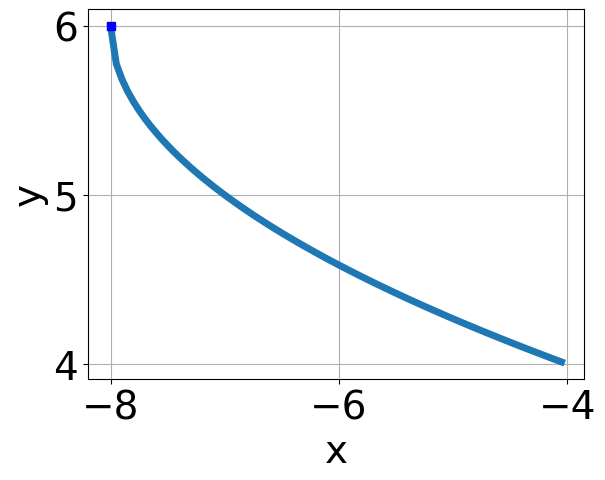
\includegraphics[width = 0.3\textwidth]{../Figures/radicalEquationToGraphCopyAB.png}\item 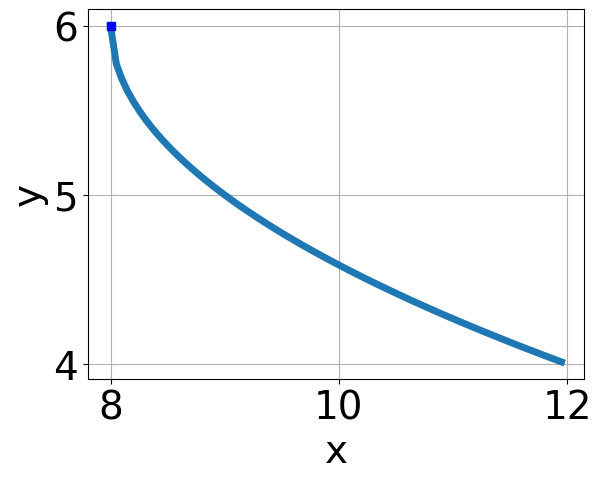
\includegraphics[width = 0.3\textwidth]{../Figures/radicalEquationToGraphCopyBB.png}\item 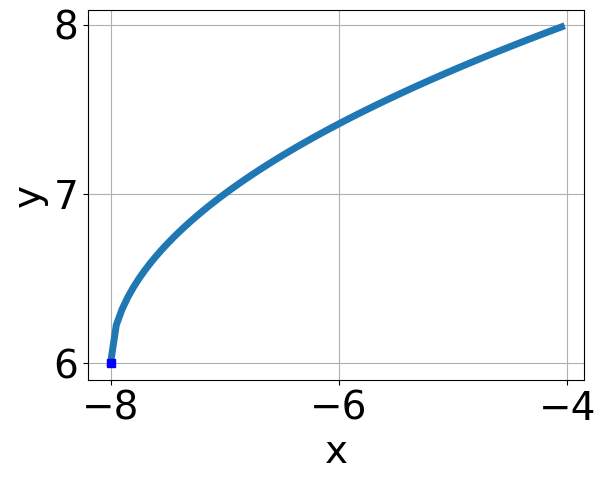
\includegraphics[width = 0.3\textwidth]{../Figures/radicalEquationToGraphCopyCB.png}\item 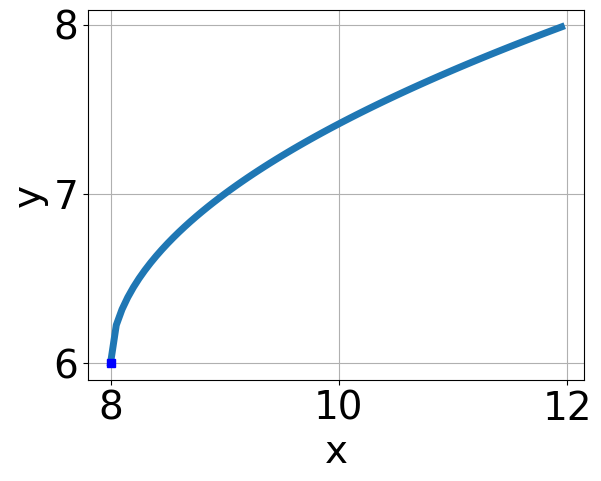
\includegraphics[width = 0.3\textwidth]{../Figures/radicalEquationToGraphCopyDB.png}\end{multicols}\item None of the above.
\end{enumerate} }
\litem{
Solve the radical equation below. Then, choose the interval(s) that the solution(s) belongs to.\[ \sqrt{9 x - 3} - \sqrt{-4 x + 3} = 0 \]\begin{enumerate}[label=\Alph*.]
\item \( x_1 \in [0.12, 0.44] \text{ and } x_2 \in [-0.12,0.69] \)
\item \( \text{All solutions lead to invalid or complex values in the equation.} \)
\item \( x \in [-0.18,0.07] \)
\item \( x_1 \in [0.12, 0.44] \text{ and } x_2 \in [0.68,1.53] \)
\item \( x \in [0.45,0.5] \)

\end{enumerate} }
\litem{
Solve the radical equation below. Then, choose the interval(s) that the solution(s) belongs to.\[ \sqrt{-4 x - 7} - \sqrt{9 x - 4} = 0 \]\begin{enumerate}[label=\Alph*.]
\item \( x \in [-0.73,0.25] \)
\item \( \text{All solutions lead to invalid or complex values in the equation.} \)
\item \( x_1 \in [-2.7, -1.21] \text{ and } x_2 \in [-0.2,1.6] \)
\item \( x \in [-1.04,-0.4] \)
\item \( x_1 \in [-2.7, -1.21] \text{ and } x_2 \in [-0.76,0.27] \)

\end{enumerate} }
\end{enumerate}

\end{document}